\section{Dini Permata Putri | 1174055}
\subsection{LeafletJS dan Mapproxy}
\begin{enumerate}
\item Pertama,run terlebih dahulu map proxy nya. Untuk ngerun nya sama seperti pada tugas sebelumnya. Untuk lebih jelasnya dapat dilihat pada gambar berikut:
\hfill\break
\begin{figure}[H]
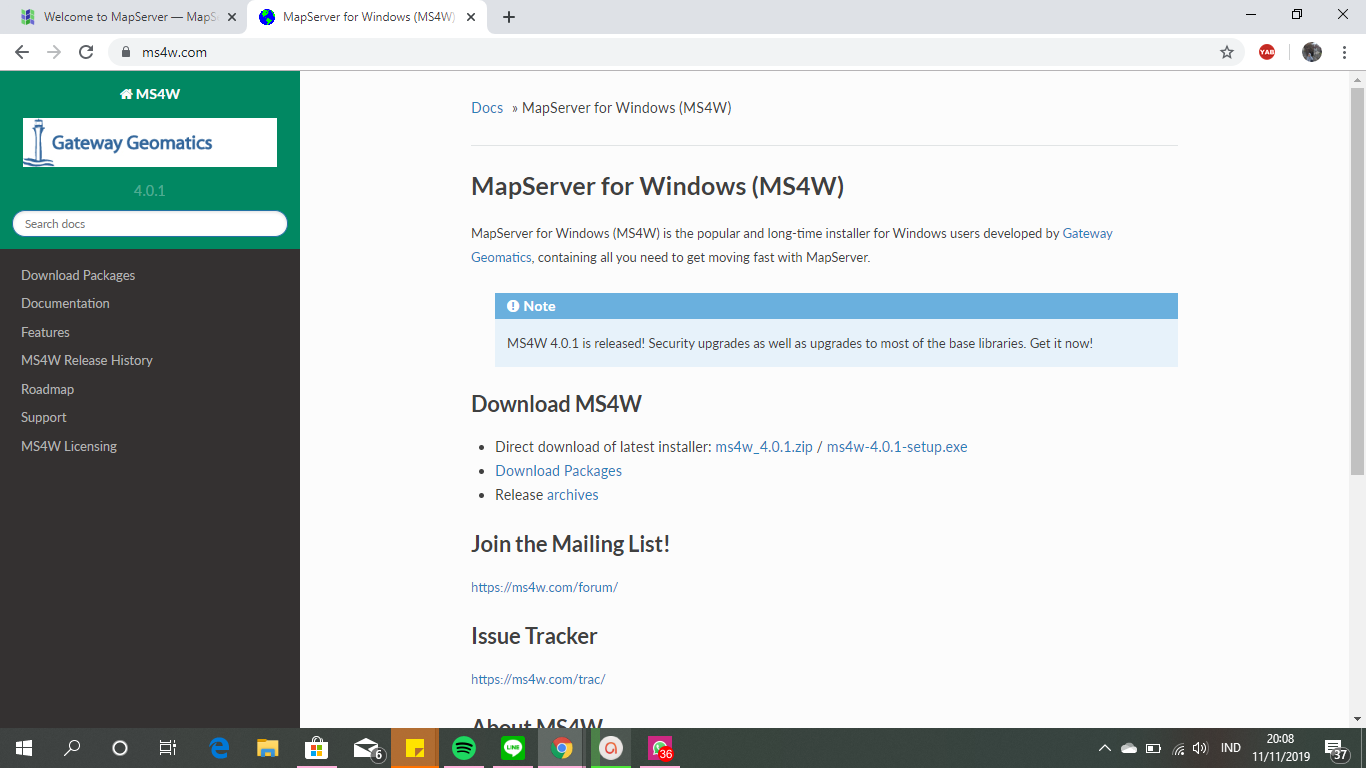
\includegraphics[width=4cm]{figures/tugas5/1174053/1.png}
\centering
\caption{Run Mapproxy}
\end{figure}
    
\item Selanjutnya, buka contoh file leafletjs yang sudah kita download sebelumnya yang berada didalam folder gede. 
\hfill\break
\begin{figure}[H]
\includegraphics[width=4cm]{figures/tugas5/1174053.png}
\centering
\caption{Isi Basic.htm}
\end{figure}
    
\item Kemudian buka browser, dan jika berhasil maka hasilnya akan seperti pada gambar berikut :
\hfill\break
\begin{figure}[H]
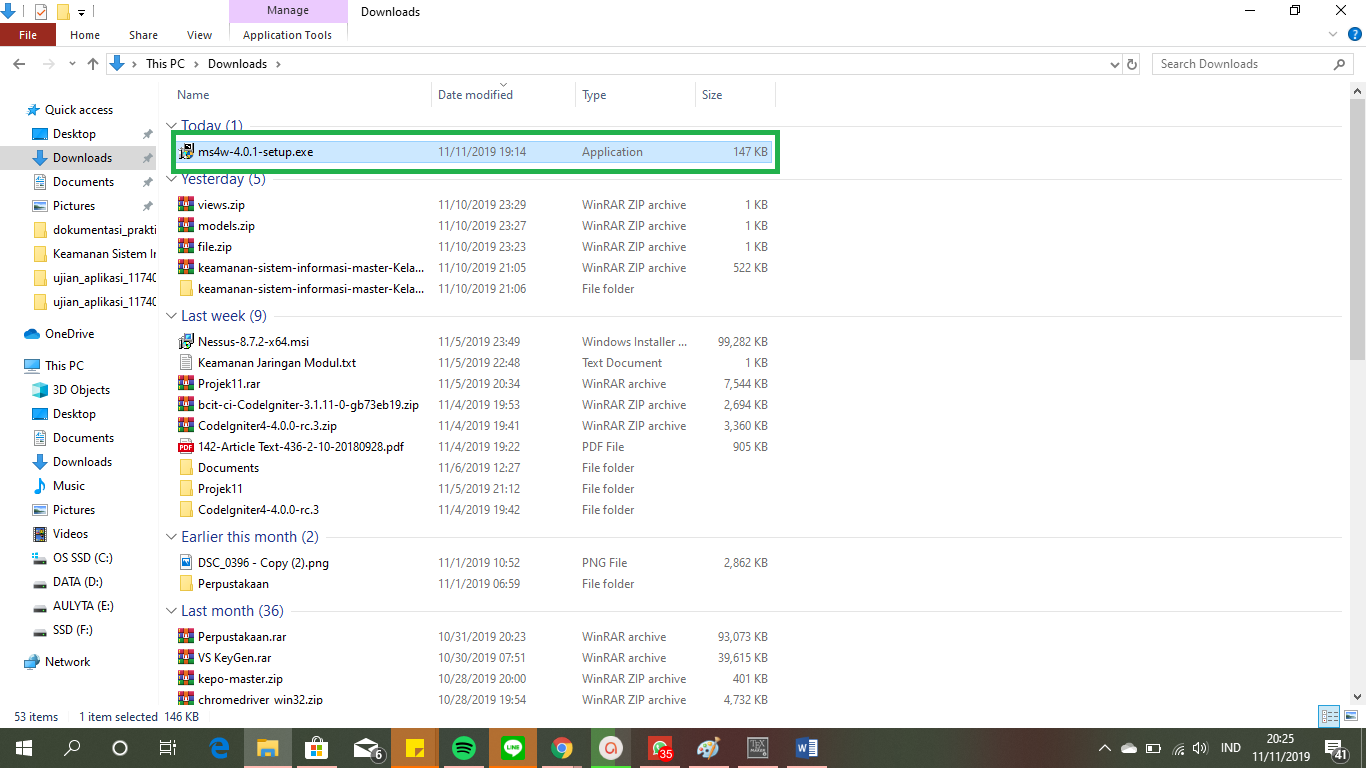
\includegraphics[width=4cm]{figures/tugas5/1174053/3.png}
\centering
\caption{Hasil dari Basic.html}
\end{figure}
  
\item Dengan menggunakan LeafletJS kita dapat menambahkan marker, circle dan polygon yaitu dengan cara seperti gambar dibawah ini, contoh ini diambil dari file marker.html yang berada didalam folder gede.
\hfill\break
\begin{figure}[H]
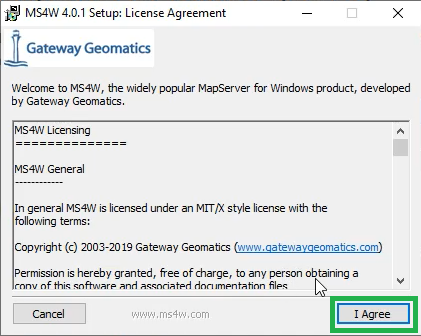
\includegraphics[width=4cm]{figures/tugas5/1174053/4.png}
\centering
\caption{Isi dari marker.html}
\end{figure}
  
\item kemudian buka filenya di browser, hasilnya seperti gambar dibawah ini.
\hfill\break
\begin{figure}[H]
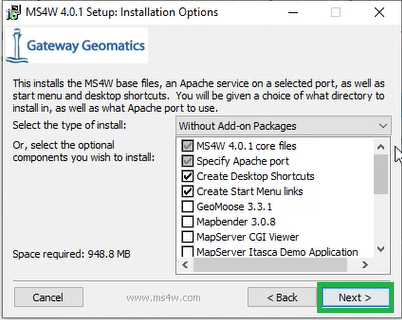
\includegraphics[width=4cm]{figures/tugas5/1174053/5.png}
\centering
\caption{Isi dari marker.html}
\end{figure}

\end{enumerate}

\subsection{Link Youtube LeafletsJS}
https://youtu.be/pBx5bSk2lmI